% ============================================================
%  SYSTEM BLOCK DIAGRAM — 5 columns + injury detection + web UI
% ============================================================
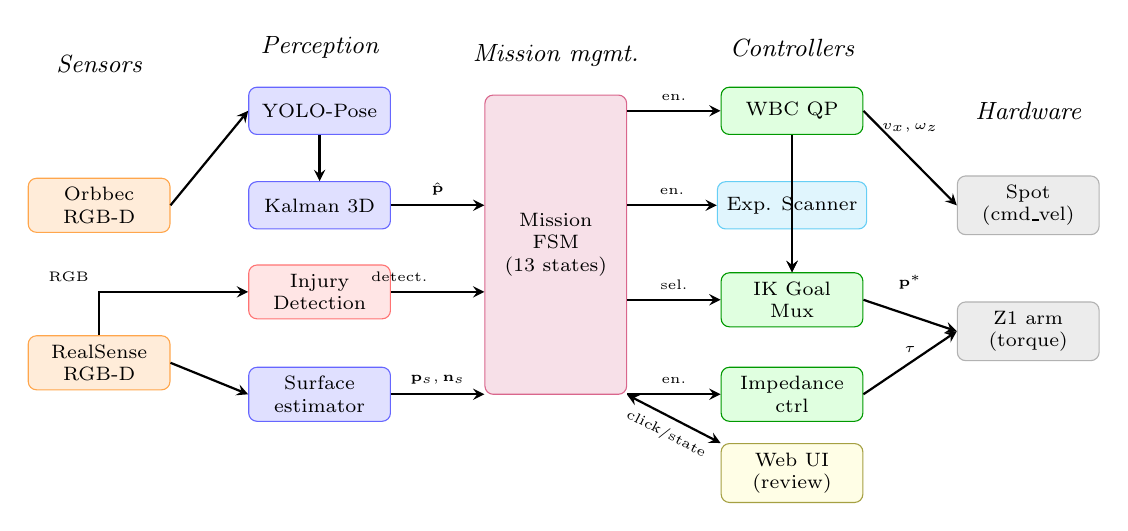
\begin{tikzpicture}[
    >=stealth,
    arr/.style    = {->, thick},
    arrb/.style   = {<->, thick},
    box/.style    = {rectangle, draw, rounded corners=3pt,
                     minimum width=1.8cm, minimum height=0.60cm,
                     font=\scriptsize, align=center, fill=white},
    sensor/.style = {box, fill=orange!15, draw=orange!70},
    percep/.style = {box, fill=blue!12,   draw=blue!60},
    injury/.style = {box, fill=red!10,    draw=red!55},
    fsmbox/.style = {box, fill=purple!12, draw=purple!60,
                     minimum width=1.8cm, minimum height=3.8cm},
    ctrl/.style   = {box, fill=green!12,  draw=green!60!black},
    expctrl/.style = {box, fill=cyan!12,  draw=cyan!60},
    web/.style    = {box, fill=yellow!10, draw=yellow!60!black},
    hw/.style     = {box, fill=gray!15,   draw=gray!60},
    lbl/.style    = {font=\small\itshape},
  ]

  % ── Column x: 0  2.8  5.8  8.8  11.8 ───────────────────────
  % ── Row y:  top rows between +2.6 and -2.4 ────────────────

  % SENSORS
  \node[sensor] (orb)  at ( 0.0,  1.0) {Orbbec\\RGB-D};
  \node[sensor] (rs)   at ( 0.0, -1.0) {RealSense\\RGB-D};

  % PERCEPTION
  \node[percep] (yolo) at ( 2.8,  2.2) {YOLO-Pose};
  \node[percep] (kf)   at ( 2.8,  1.0) {Kalman 3D};
  \node[injury] (inj)  at ( 2.8, -0.1) {Injury\\Detection};
  \node[percep] (surf) at ( 2.8, -1.4) {Surface\\estimator};

  % FSM
  \node[fsmbox] (fsm)  at ( 5.8,  0.5) {Mission\\FSM\\(13 states)};

  % CONTROLLERS
  \node[ctrl]  (wbc)  at ( 8.8,  2.2) {WBC QP};
  \node[expctrl] (exp) at (8.8,  1.0) {Exp. Scanner};
  \node[ctrl]  (mux)  at ( 8.8, -0.2) {IK Goal\\Mux};
  \node[ctrl]  (imp)  at ( 8.8, -1.4) {Impedance\\ctrl};

  % WEB UI
  \node[web] (webui) at ( 8.8, -2.4) {Web UI\\(review)};

  % HARDWARE
  \node[hw] (spot) at (11.8,  1.0) {Spot\\(cmd\_vel)};
  \node[hw] (z1)   at (11.8, -0.6) {Z1 arm\\(torque)};

  % ── Sensors → Perception ────────────────────────────────────
  \draw[arr] (orb.east)  -- (yolo.west);
  \draw[arr] (yolo.south) -- (kf.north);
  \draw[arr] (rs.east)   -- (surf.west);
  \draw[arr] (rs.north)  |- node[above left,font=\tiny]{RGB} (inj.west);

  % ── Perception → FSM ────────────────────────────────────────
  \draw[arr] (kf.east)   -- node[above,font=\tiny]{$\hat{\mathbf{p}}$}
             (fsm.west |- kf);
  \draw[arr] (inj.east)  -- node[above left,font=\tiny]{detect.}
             (fsm.west |- inj);
  \draw[arr] (surf.east) -- node[above,font=\tiny]{$\mathbf{p}_s,\mathbf{n}_s$}
             (fsm.west |- surf);

  % ── FSM → Controllers ───────────────────────────────────────
  \draw[arr] (fsm.east |- wbc) -- node[above,font=\tiny]{en.} (wbc.west);
  \draw[arr] (fsm.east |- exp) -- node[above,font=\tiny]{en.} (exp.west);
  \draw[arr] (fsm.east |- mux) -- node[above,font=\tiny]{sel.}(mux.west);
  \draw[arr] (fsm.east |- imp) -- node[above,font=\tiny]{en.} (imp.west);

  % ── WBC → Mux + Exp Scanner → Mux ──────────────────────────
  \draw[arr] (wbc.south) -- (mux.north);
  \draw[arr] (exp.south) -- (mux.north);

  % ── FSM ↔ Web UI ────────────────────────────────────────────
  \draw[arrb] (fsm.south east) -- node[below,font=\tiny,sloped]{click/state} (webui.north west);

  % ── WBC → Spot ──────────────────────────────────────────────
  \draw[arr] (wbc.east) --
           node[above,font=\tiny,yshift=2mm]{$v_x,\omega_z$} (spot.west);

  % ── Mux → Z1 ────────────────────────────────────────────────
  \draw[arr] (mux.east) --
             node[above,font=\tiny,yshift=2mm]{$\mathbf{p}^*$}
             (z1.west);

  % ── Imp → Z1 ────────────────────────────────────────────────
  \draw[arr] (imp.east) --
             node[above,font=\tiny]{$\boldsymbol{\tau}$}
             (z1.west);

  % ── Column labels ────────────────────────────────────────────
  \node[lbl] at ( 0.0,  2.8) {Sensors};
  \node[lbl] at ( 2.8,  3.0) {Perception};
  \node[lbl] at ( 5.8,  2.9) {Mission mgmt.};
  \node[lbl] at ( 8.8,  3.0) {Controllers};
  \node[lbl] at (11.8,  2.2) {Hardware};

\end{tikzpicture}
